\section{The Source of Approximation Bias}
\label{sec:source-of-bias}

To calculate an estimate of $f_i$, the level $w^*$ is chosen
to maximize $t_i^{(w)}$ -- the number of collision-free counters with value $i$ at level $w$.

$$t_i^{(w)} = |\{T_w[c].v = i ~|~ c \in \{0, \dots, r-1\}\}| ~~~~~~~~~~~~ w^* = \arg\max_w t_i^{(w)}$$

Then the number of counters at this level is converted into the estimate of $f_i$ by multiplying it by 
$2^{w^*} \cdot \left(1 - \frac{1}{r}\right)^{1 - F_0/2^{w^*}}$. 

The reason why the level $w^*$ is selected as it is, is not clearly stated in Kmerlight's original paper \cite{Sivadasan2016}. 
We believe that the authors hoped to minimize the variance of the estimator $\hat f_i$.

\subsection{Collision-free Counters and Analytical $w^*$}
\label{sec:analytical-w}
Let us first revise that by the term $k$-mer we understand a string of $k$ characters. A $k$-mer may occur multiple times in an input stream. 
If it occurs $i$ times, we say its abundance is $i$. If counter $T_w[c]$ holds value $i$, it means that $i$ occurences of the same $k$-mer were hashed into it.
We assume that all the collisions are being detected, so the value of the counter equals the abundance of the $k$-mer hashed into it.

Can the level $w^*$ be computed analytically? This level should maximize $E(t_i^{(w)})$, the expected number of collision-free counters holding the value $i$.

But the values $E(t_1^{(w)}), E(t_2^{(w)}), \dots, E(t_m^{(w)})$ are in the same relative ratios at every level. If there are two times more $k$-mers with
abundance one than the $k$-mers with abundance three, we can also expect two times more counters storing the value one than there are counters storing value three.
By this argument, maximizing $E(t_i^{(w)})$ means maximizing the number of all collision-free counters at one level.

Let us denote with $p_{cf}$ the probability that a single counter is collision-free. Then the expected number of collion-free counters is $r \cdot p_{cf}$.
Under the assumption of uniform hashing into one of $r$ counters, $p_{cf}$ is the probability that only one of $F_0/2^w$ $k$-mers were hashed into that counter.

The number of distinct $k$-mers hashed into one counter ($X$) follows a binomial distribution, $X \sim \mathrm{Bin}(F_0/2^w, 1/r)$, so $p_{cf}$ can be expressed as follows:
\begin{equation} \label{eq:pcf}
p_{cf} = P[X=1] = \frac{F_0}{2^w} \cdot \frac{1}{r} \left(1 - \frac{1}{r}\right)^{F_0/2^w - 1}
\end{equation}
and the probability that a counter is empty ($p_e$) and the probability that a counter holds a collision ($p_c$) can be derived easily as well:
$$p_e = P[X=0] = \left(1 - \frac{1}{r}\right)^{F_0/2^w} ~~~~~~ p_c = P[X>1] = 1 - p_e - p_{cf}$$

The value of $w^*$ can be obtained by differentiation ($\frac{\mathrm{d}}{\mathrm{d}w}p_{cf} = 0$) or by using the discrete inequalities 
$p_{cf}^{(w^*)} \geq p_{cf}^{(w^*-1)}, p_{cf}^{(w^*)} \geq p_{cf}^{(w^*+1)}$. 
By manipulating the inequalities we get
\begin{equation} \label{eq:wstarbounds}
\frac{1}{4} \leq \left(1 - \frac{1}{r}\right)^{F_0/2^w} \leq \frac{1}{2}
\end{equation}

\medskip

Apart from our ability to calculate $w^*$ and $p_{cf}$, an important outcome of
this section is the observation that the value $w^*$ selected by Kmerlight should not
depend on $i$ or $f_i$ and it is expected to be the same for the estimates of all $f_i$.

\subsection{The Problematic Data}
Kmerlight guarantees precise estimation for $f_i$ with values close to $F_0$.
Unfortunately, in the sequencing data, values of $f_i$ for $i > 1$ are considerably 
smaller than $F_0 \sim f_1$. This is mainly caused by sequencing errors and also
by the nature of the histogram.

With sequencing error rate of 2\%, 35\% $k$-mers are erroneous and thus unique with high probability.
As an effect 35\% of all $k$-mers are concentrated in $f_1$ and 65\% of $k$-mers are
distributed to other $f_i$. With coverage $c$ the histogram is expected to have 
approximately $c$ columns which makes $f_2, \dots, f_c$ smaller than $f_1$ by an order of magnitude if the coverage is in order of tens.

The second effect that makes values $f_i$ of higher $i$ smaller, is that to increase 
$f_1$ only one $k$-mer is needed, but to increase $f_{10}$ by one, ten occurences of
 the same $k$-mer must be added to the input stream.

These two effects combined explain, why is the value $f_1$ a hundred times larger than
the values of $f_i, i>10$ in the presented experimental data in figures
\ref{img:exact-vs-approximated-histogram} and \ref{img:exact-vs-approximated-histogram-log}.

\subsection{Explanation of Bias}
Since the ratio $f_i / F_0$ is very low for $i>1$ and this ratio determines
the fraction of collision-free counters holding the value $i$, each $f_i$ is
represented by only a relatively small number of collision-free counters at each level of 
Kmerlight's sketch. Let us denote as $t^{(w)}$ the observed number of all collision-free
counters at the level $w$ and denote as $t_i^{(w)}$ the number of those with value $i$.

The expected number of collision-free counters at level $w$ is 
$E(t^{(w)}) = r \cdot p_{cf} = F_0 / 2^w \cdot (1 - 1/r)^{F_0/2^w - 1}$ from \ref{eq:pcf}.
From the bounds \ref{eq:wstarbounds} we know that at level $w^*$
$1/4 \leq (1 - 1/r)^{F_0/2^{w^*}} \leq 1/2$.

By examining the levels $w^*-1$ and $w^*+1$ we learn that the number of collision-free counters at these levels is similar to the number of collision-free counters at level $w^*$. There are two times more $k$-mers hashed into the level $w^*-1$ and 2-4 times more collisions happen. Similarly, two times fewer $k$-mers are hashed to the level $w^*+1$ but 2-4 times less collisions happen.

As a result of high variance of $t_i^{(w)}$ and close values of $E(t^{(w^*-1)}), 
E(t^{(w^*)}),E(t^{(w^*+1)})$, any of these levels could hold the maximal $t_i^{(w)}$ 
and become chosen by Kmerlight as its $w^*$. Kmerlight always chooses the level which 
maximizes $t_i^{(w)}$ and this leads to values of $t_i^{(w^*)}$ consistently higher
than $E(t_i^{(w^*)})$ and consequently biases the estimator $\hat f_i$.

\subsection{Demonstration on Experimental Data}

In order to demonstrate the similarity of $E(t^{(w)})$ at the levels close to $w^*$ we
display the values of $p_{cf} = E(t^{(w)}) / r, p_e, p_c$ for different levels in
figure \ref{img:pe-pcf-pc}. These probabilities represent the fractions of 
collision-free, empty and collided counters respectively. 

\begin{figure}
\centerline{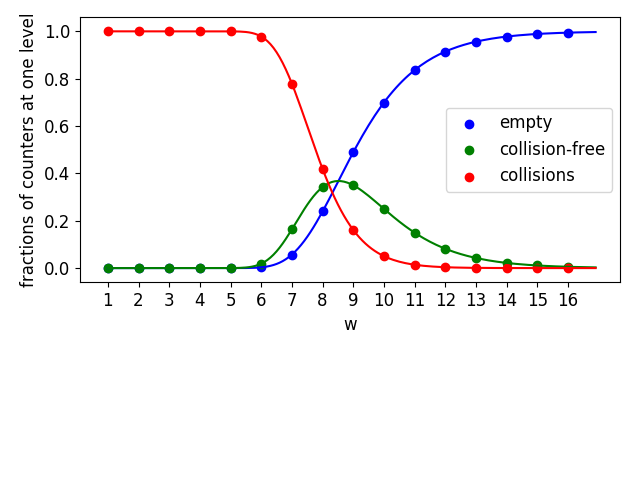
\includegraphics[width=0.8\textwidth, trim={0cm, 3.5cm, 0cm, 0cm}, clip]{images/pcf.png}}
\caption[Plot of $p_e, p_{cf}, p_c$ across the levels]{The values of $p_e, p_{cf}, p_c$ 
represent the theoretical fractions of empty, collision-free and collided counters in
each level respectively. To relate these theoretical values to the experiment we set 
$F_0 = 1.2 \times 10^7, r = 2^{15}$. The presented experiment shows the worst possible
situation with $E(t^{(8)}) \approx E(t^{(9)})$.}
\label{img:pe-pcf-pc}
\end{figure}

From one Kmerlight run we extracted the values $w^*$ for different $f_i$ and we present them in the figure \ref{img:w-selected-by-kmerlight}.

\begin{figure}
\centerline{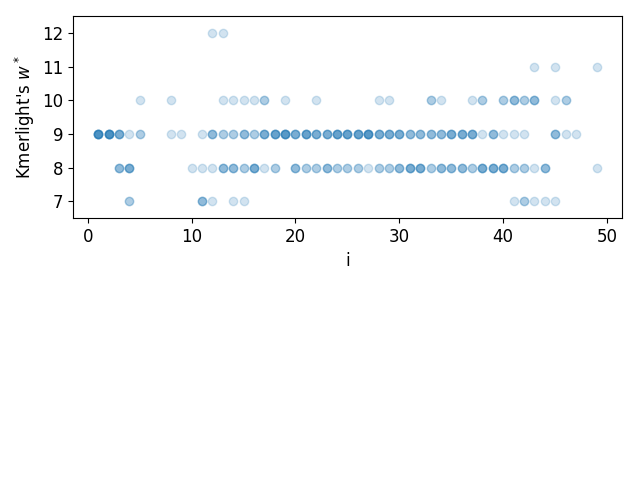
\includegraphics[width=0.8\textwidth, trim={0cm, 5.5cm, 0cm, 0cm}, clip]{images/kmerlight_wstar.png}}
\caption[$w^*$ selected by Kmerlight]{For estimate of each $f_i$ there are up to seven
values of $w^*$, each selected by one instance of seven Kmerlight's sketches. The most of 
selected levels follow the analytical $w^* = 9$, however, Kmerlight often chooses 
$w^* = 8, 10$ to maximize $t_i^{(w^*)}$. Note that for $3\leq i \leq 15$ and $i \geq 40$
are the values of $f_i$ low and thus $t_i^{(w)}$ has high variance. The maximal
$t_i^{(w)}$ can also be reached at levels more distant from the analytical $w^* = 9$.}
\label{img:w-selected-by-kmerlight}
\end{figure}
